%%%%%%%%%%%%%%%%%%%%%%%%%%%%%%%%%%%%%%%%%%%%%%%%%%%%%%%%%%%%%%%%%%%%%%%%%%%%%%%%
%2345678901234567890123456789012345678901234567890123456789012345678901234567890
%        1         2         3         4         5         6         7         8
%% memo.tex
%% V1.0
%% 2015/09/20
%% by Prof. Rui Santos Cruz
%% based on a template created by Rob Oakes
%%%%%%%%%%%%%%%%%%%%%%%%%%%%%%%%%%%%%%%%%%%%%%%%%%%%%%%%%%%%%%%%%%%%%%%%%%%%%%%%
\documentclass[a4paper,12pt]{texMemo}
% --> Please Choose the MAIN LANGUAGE for the document in package BABEL
% --> by replacing "main=" in language name selector. Default is "main=english"
\usepackage[main=english,portuguese]{babel} % Defines Main language
\usepackage[utf8]{inputenc}
\usepackage{iflang}
\usepackage{ifthen}
\usepackage{parskip}
\usepackage{amsthm}
\usepackage{amsmath}
\setlength{\parindent}{15pt}
\logo{
\includegraphics[width=0.3\textwidth]{madison.jpg}} % Logo
%%%%%%%%%%%%%%%%%%%%%%%%%%%%%%%%%%%%%%%%%%%%%%%%%%%%%%%%%%%%%%%%%%%%%%%%%%%%%%%%
%	MEMO INFORMATION --> Write your info in the following tags.
%%%%%%%%%%%%%%%%%%%%%%%%%%%%%%%%%%%%%%%%%%%%%%%%%%%%%%%%%%%%%%%%%%%%%%%%%%%%%%%%
\memofrom{Luxi Cao, Zongyan Wang} % Sender(s) Name
\memocourse{Stat 992: Dependence Modeling with Copulas} % Course Name, or abbreviated acronym
\memosubject{Lecture 7 Scribe} % Subject
\memodate{\today} % Date, -> set to \today for automatically print todays date
%%%%%%%%%%%%%%%%%%%%%%%%%%%%%%%%%%%%%%%%%%%%%%%%%%%%%%%%%%%%%%%%%%%%%%%%%%%%%%%%
\begin{document}
\maketitle % Print the memo header information
%%%%%%%%%%%%%%%%%%%%%%%%%%%%%%%%%%%%%%%%%%%%%%%%%%%%%%%%%%%%%%%%%%%%%%%%%%%%%%%%
%	MEMO CONTENT --> Your content is written here
%%%%%%%%%%%%%%%%%%%%%%%%%%%%%%%%%%%%%%%%%%%%%%%%%%%%%%%%%%%%%%%%%%%%%%%%%%%%%%%%
\section{Q \& A}
Q1. How to relate infinitely divisible, domain of attraction, stable, slowly varying?
\begin{enumerate}
\item In case of multivariate distribution F, as long as $F^q, q>0$, F is infinitely divisible. if q is a positive integer, then it is always true. Otherwise, you have to check the power function.
In probability theory, a probability distribution is infinitely divisible if it can be expressed as the probability distribution of the sum of an arbitrary number of independent and identically distributed random variables. 
\item Domain of attraction: Limit distribution of Minimum or Maximum of random variables exists
\item Sum stable: For any distribution, if a random variable can be expressed as a linear combination of independent variables. Those random variables follow the same distribution family.
\item Max stable: take the maximum of a number of random variables. The random variable has a limit distribution with indivisible property. Any of these multivariate extreme value distribution can be expressed as a linear combination of unit $Fr\acute{e}chet$ random variables.
\item slowly varying: many of those joint survival distribution can be expressed as $\bar{F}(x) \sim x^{-\alpha} L(x)$
\end{enumerate}

Q2. Tow-stage estimation for copula models, why a big difference between $\hat{\eta}$ and $\tilde{\eta}$, relative to the standard errors for V, suggests either the copula model or the uni-variate models may be inadequate. How 'big' is a relative big?
\begin{enumerate}
\item If our estimation procedure is consistent then both good enough. This is so called consistency check: $\hat{\eta}$ and $\tilde{\eta}$ should not differ a lot.
\item Some people dislike 2 stage, because after you estimate the first part, there is a random variable. Then you have to adopt return part. Then the second part automatically isn't good.
\item Coordinate decent is more popular recently, estimate the parameter one by one. 
\item How big is a relative big? Ex. in linear regression model, how to consider two variances are the same? Rule of Thumb: $\hat{\eta}$/$\tilde{\eta}$ $\in [0.5, 2]$
\end{enumerate}

Q3. How to use Laplace transformation to construct a copula can be further studied. Chap3 would talk about it.

Q4. Using frailty parameter and resilience parameter, we can have Archimedean copulas. What is the importance of Archimedean copula?

Archimedean Copula's property will be shown. Archimedean Copula is a very broad family. Many of copulas dependence structures could be constructed with the help of Archimedean Copula. it generates Gumbel Copulas which is extreme value copula.

Q5. Is there any formal definition of concordance ordering? since the concordance ordering is a way to compare multivariate distributions with the same set of uni-variate margins, but usually what we know is joint distribution rather than marginal distribution. So how do we apply this to practice problem?

\begin{enumerate}
\item The first part is discussed in Section 2.9
\item Second part: Partly agree with what we know is joint distribution rather than marginal distribution. If we consider Multi-Normal, then it is the case. 
\item The reason for we study Copulas dependence is that we don't have unified parametric form to model everything. Since in many cases, those marginal distributions are not within the same family. 
\item For those marginal distribution, we always could do some transformations. Firstly, we fit some distribution to the marginal, then transform to uniform or $Fr\acute(e)chet$, then we use joint structure to model the joint distribution. This is the sample statement.
\item Applications will be shown
\end{enumerate}

Q6. In the slides, there is one paragraph said that: 
"The concordance ordering is a way to compare multivariate distributions with the same set of univariate margins so that we can decide if one multivariate distribution represents more dependence that another."
I wonder how to use the concordance ordering?

It will be taught soon. Be patient little little baby.

Q7. Text p28: "2.1.2 Absolutely continuous and singular components". It says: "The decomposition could also be written in terms of survival functions." Could you please explain more about this?

Note $F = \delta_{ac}F_{ac} + \delta_{sin}F_{sin} + \delta_{d}F_d$ could be written in terms of survival function:
$1 - F = \bar{\delta}_{ac}(1 - F_{ac}) + \bar{\delta}_{sin}(1 - F_{sin}) + \bar{\delta}_{d}(1 - F_d)$. Those three delta are different.

Q8. Could you please talk more about Vine Copulas on Friday, 1) Why is partial correlation important for vine copula, 2) How can we do the pair-copula construction in general, 3) How could we estimate a pair-copula when we have the given data.

Will be taught later


Q9. You mentioned when we have multiple responses and common covariates we can apply copula regression. Can you give an example of that?

\begin{enumerate}
\item eg:
$Y=(y_1,y_2,....,y_d)^T$ , $x_1, x_2, ..., x_p$ covariates. $y_1, ..., y_d$ are in the same distribution family.
How could we do copulas regression? \
Suppose we want to model $y_1$ to $y_d$ to a Gumbel Copula. Gumbel Copula only has one parameter $\lambda$. This $\lambda$ could be expressed as a function of X: \
$\lambda(x_1,x_2,x_3,..,x_p)=f(a_1x_1+a_2x_2+...a_px_p)$
\item Copula parameter is a function of covariates.
\item Think about Multivariavte-Normal, in our multi-variate linear regression, choose $\lambda$ as $\mu$ would be the same thing.
\end{enumerate}

Q10. Can you talk more about concordance ordering? How can it cover the dependence information?

Will be taught soon.

Q11. How to compare copula and multivariate models? When should we use copula?

\begin{enumerate}
\item In general, in multivariate distribution we have same marginals, basically, you could call it as Copulas too.
\item We could use Copulas in any time. A specific reason for using Copulas is when we transform all the marginals to the same distribution, either uniform distributed or unique $Fr\acute{e}chet$. Some of people in UK transform the marginal to Gumbel distributed.  
\end{enumerate}

Q12. What is slowly varying function? What's its properties?

$\frac{l(tx)}{l(x)}$ has a limit 1. eg. constant function, $\log(x)$ is slowly varying function. 

Q13. Can you talk more about stochastic positive dependence?

We will talk about it. 

Q14. If we estimate the three distinct regions of the composite empirical CDF, for the interior, upper and lower tails, then we can graphically concatenate and display the result. But how can we assess the model fit?

3 distinct regions:
\begin{enumerate}
\item In general linear regression, many situations we always have some good model fitting. 
\item Ratio estimation procedure, good estimation at upper tail, but not in the middle. No concrete answer.
\item Extreme dependence no much attention to the middle part.
\item Regression pay attention to the middle part, the middle part dominates the fitting procedure. 
\item We don't use residual, we check misclassification rate. 
If you generate data using the hyper-plane,. either solution is acceptable for classification. 
\end{enumerate}

Q15. Vine copulas were mentioned in Section 2.6. Given data, how can we estimate a pair-copula(if we focus on bivariate copulas) decomposition and represent it with regular vine structure?

We will discuss in Chapter 4.

Q16. Does there exist a multivariate distribution on the positive quadrant that has tractable higher order moments? 

\begin{enumerate}
\item All the multivariate- Normal, multivariate- T have high order moment
\item Copulas transform marginal random variables to uniform, which means all the high order moment exist.
\end{enumerate}

Q17. What unconditional copulas should be chosen to approximate the conditional copulas?

\begin{enumerate}
\item Conditional Copula is a copula we choose in constraint of a subset. The family of the copulas are unconditional copulas. 
\item Up to our purpose.
\end{enumerate}

Q18. I am interested in the effect of truncation/ censoring on dependence.
For example, when one variables has upper-tail censoring, then potential upper-tail dependency may be hidden.

\begin{enumerate}
\item Truncation: Observe the value under the threshold. See Figure 1
\item If when the data observed, the data is not truncated or censored, we can just fit the model to original data.
Then you can apply truncation, then study joint structure. 
\item Truncation,Censoring applies to univariate marginals. (Research question) 
\item Tail dependence: $P(X>u|Y>u)$. Suppose we have bivariate-normal or bivariate-T,  $lim_{u->u^*}P(X^*>u|Y^*>u)=\lambda$. Would be a research question for whether $\lambda$ is equal to 0. Where $X^*=min{X,u^*},Y^*=min{Y,u^*}$   
\end{enumerate}
\begin{figure}
\centering
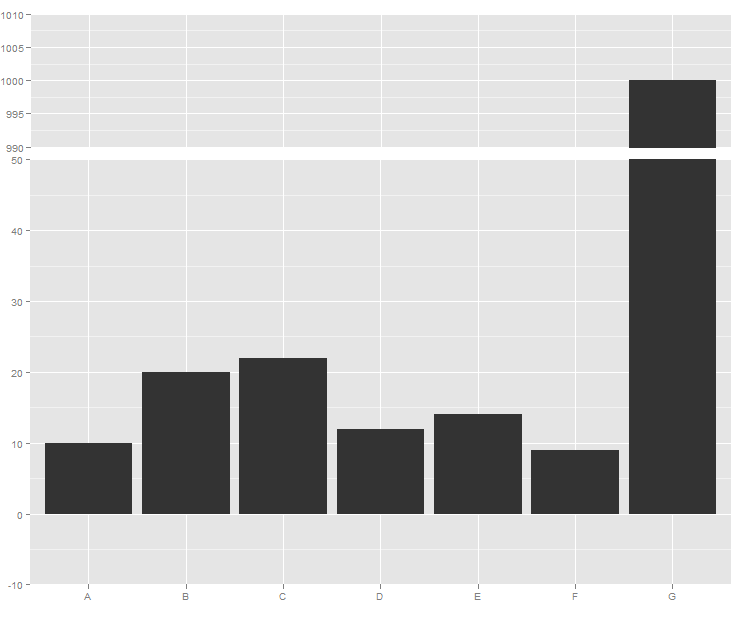
\includegraphics[width=0.5\textwidth]{truncate.png}
\caption{\label{fig: Example of Data Truncation} Data Truncation: Values Observed under the threshold}
\end{figure}


Q19. Effect of mis-specification of the marginal model, on the dependence parameter estimated from either an IFM or full-likelihood approach to estimating copula parameters?

There is effect of mis-specification. How serious depends on the model itself. We add some estimation procedure called Cauchy likelihood or pseudo likelihood.


Q20. Effect of truncation and censoring, on the dependence parameter? What happens, if we ignore truncation? What happens, if we ignore censoring?

\begin{enumerate}
\item Truncation and censoring effect: Research question more like survival analysis part.
\item Basically, truncation and censoring are different. If we treat truncated data as normal distribution and transform it to uniform distribution, then we don't know what will happen yet. It also depends on the types of model we have. It's good research question. 
\end{enumerate}

Q21. I found some papers about tail conditional variance. Would be interested to have similar studies for extreme value distributions. How to apply Laplace transformation to construct copula?

We could do research in this direction.

Q22. In the book 2.9, $Fr\acute{e}chet$ class was not clearly defined. What is the definition of $Fr\acute{e}chet$ class?

\begin{enumerate}
\item $Fr\acute{e}chet$ class: A $Fr\acute{e}chet$ class collects all multivariate joint distribution functions that have the same marginals.
\item Upper bound: always is a joint distribution, lower bound: not always a joint distribution
\end{enumerate}

\section{Some Notes for the lecture}
1. Linear coefficient may not be a good one. see Figure 2
\begin{figure}
\centering
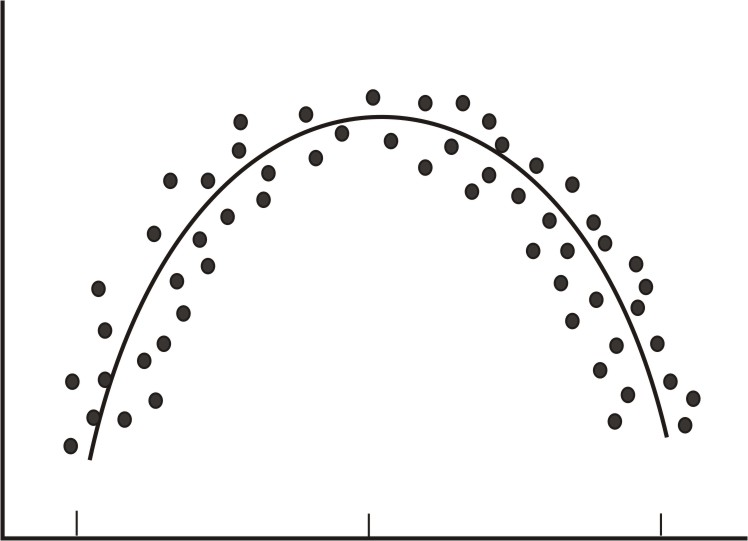
\includegraphics[width = 0.5\textwidth]{nonlinear.png}
\caption{\label{fig: non-linear correlation}May suggests $y \sim x^2$, but correlation coefficient will be approximately 0}
\end{figure}

2. Example 2.7 Suppose $X_1 \sim Pareto(\alpha, 1)$, and $X_2 \sim Exponential(1)$, then $X_2 = F_2^{-1}(F_1(X_1)) = -\log[(1+X_1)^{-\alpha}] = \alpha \log(1+X_1)$ is a monotone increasing functional relation but the correlation of $X_1$, $X_2$ is not 1.
\begin{proof}
$X1 = e^{X_2/\alpha} - 1, X_2 \sim Expo(1)$
\begin{align*}
Cov(X_1, X_2)
& = \int_0^{\infty} x(e^{x/\alpha} - 1) e^{-x} dx\\
& = \int_0^{\infty} x e^{-\frac{\alpha - 1}{alpha}x} - x e^{-x} dx\\
& = (\frac{\alpha - 1}{\alpha})^2 - 1 \\
& = \frac{2\alpha - 1}{(\alpha - 1)^2}
\end{align*}
Since $X_1 \sim Pareto(\alpha, 1)$, and $X_2 \sim Exponential(1)$, we have $var(X_1) = 1$, $var(X_2) = \frac{\alpha}{(\alpha - 1)^2 (\alpha - 2)}$,\\
We have $Corr(X_1, X_2) = \frac{2\alpha - 1}{(\alpha - 1)\sqrt{\alpha/(\alpha - 2)}}$
\end{proof}


%%%%%%%%%%%%%%%%%%%%%%%%%%%%%%%%%%%%%%%%%%%%%%%%%%%%%%%%%%%%%%%%%%%%%%%%%%%%%%%%
\end{document}

